\documentclass[letterpaper,11pt]{book}
\usepackage{mystyle}

% Book's title and subtitle
\title{\huge \textbf{Heat and Mass Transfer in Practice}  \large \textbf{Using Mathematica}. \footnote{This is tutorial for ME 8381.} }
% Author
\author{\textsc{John C. Bischof} \footnote{Professor in Mechanical Engineering of University of Minnesota.}
, \textsc{Feng Liu}}

\begin{document}

%remove the red rectaugular around the reference.
\hypersetup{pdfborder=0 0 0}
%\frontmatter
\maketitle
\tableofcontents
%\listoffigures
%\listoftables
%\mainmatter

%include chapters

\chapter{Introduction to Mathematica}
Mathematica, developed by Wolfram Research\footnote{Wolfram Research is a private company makes computation software}, is a computational software program used in many scientfic, engineering, mathematical and computing fields, based on symbolic mathematics. The programming language using in Mathematica is called Wolfram Language.

\section{Overview}
\subsection{Installation}
Students with a CSE Labs account could download and use \emph{Mathematica} free of charge from \href{https://wwws.cs.umn.edu/download_software/mathematica}{\textcolor{blue} {Mathematica download page}}\footnote{\url{https://wwws.cs.umn.edu/download_software/mathematica}}. By following the instructions from that page, you could install \emph{Mathematica} on Windows, Mac or Linux. 

\begin{figure}[h!]
  \centering
    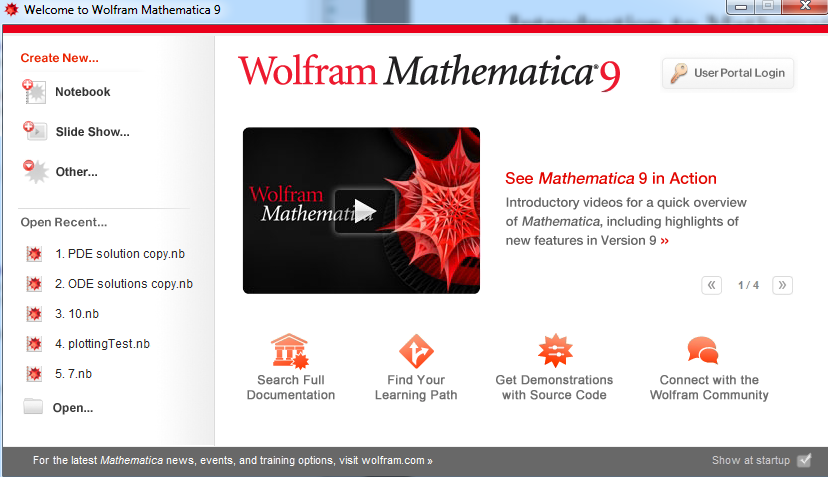
\includegraphics[scale=0.4]{figures/mathematica}
  \caption{Initialization interface of Mathematica}
  \label{fig:mathematica}
\end{figure}

\section{Tutorial}
There are many online tutorials that could help you learning \emph{Wolfram Language} and \emph{Mathematica}. You could find detailed tutorial at \href{http://reference.wolfram.com/language/?source=nav}{\color{blue} Wolfram Language \string& System Documentation Center}\footnote{\url{http://reference.wolfram.com/language/?source=nav}}. Those topics include:
\begin{itemize}
\item Core Language \string& Structure
\item Symbolic \string& Numeric Computation
\item Data Manipulation \string& Analysis
\item Visualization \string& Graphics
\item Images
\item ...
\end{itemize}

There are also many free video courses for educators and researchers which can be found at \href{http://www.wolfram.com/training/courses/edu001.html}{\color{blue} Mathematica for Teaching and Education.}\footnote{\url{http://www.wolfram.com/training/courses/edu001.html}} and
\href{http://www.wolfram.com/training/courses/edu002.html}{\color{blue} Mathematica for University Research}\footnote{\url{http://www.wolfram.com/training/courses/edu002.html}}. In the following section, we will look through some basics of \emph{Wolfram Language}.

\section{Basics}
\subsection{Simple Calculations}
In this section, we will see some examples on some basic arithmetic operations. The Wolfram Language is case sensitive. So
we should use \textbf{Sin} rather than \textbf{sin} to represent
a sinusoidal function.
\\~\\
\textbf{n = 3 + 6}\\
$9$
\\~\\
\textbf{n = 2 + 7 - 8/6}\\
$\frac{23}{3}$
\\~\\
\textbf{Sin[Pi/6]}\\
$\frac{1}{2}$
\\~\\
\textbf{n = Sin[30 Degree]}\\
$\frac{1}{2}$
\\~\\
\textbf{N [Sin[Pi/6]]}\\
$0.5$

\subsection{Matrix Operations}
Vectors and matrices in the Wolfram Language are simply represented by lists and by lists of lists, respectively.
Some basic matrix operations are as shown in Table~\ref{table:matrixOps}.
~\\\\
Expressions of a $3\times3$ matrix:\\
\textbf{m=\{\{-9,19,3\},\{-3,7,1\},\{-7,17,2\}\}}\\
\{\{-9, 19, 3\}, \{-3, 7, 1\}, \{-7, 17, 2\}\}

~\\
Transposing matrix \textbf{m}:\\
\textbf{Transpose[m]}\\
\{\{-9, -3, -7\}, \{19, 7, 17\}, \{3, 1, 2\}\}

~\\
Expressing \textbf{m} in matrix form\textbf{m}:\\
\textbf{MatrixForm[m]}\\
$\left(
\begin{array}{ccc}
 -9 & 19 & 4 \\
 -3 & 7 & 1 \\
 -7 & 17 & 2 \\
\end{array}
\right)$
\\~\\
Inversing matrix \textbf{m}:\\
\textbf{Inverse[m]}\\
$
\left(
\begin{array}{ccc}
 -\frac{3}{2} & \frac{13}{2} & -1 \\
 -\frac{1}{2} & \frac{3}{2} & 0 \\
 -1 & 10 & -3 \\
\end{array}
\right)
$

\begin{table}[H]
\caption{Basic matrix operations} % title of Table
\centering % used for centering table
\begin{tabular}{c c}
\hline %inserts double horizontal lines
Function & Purpose\\
%heading
\hline % inserts single horizontal line
Transpose[m] & Transpose $m^T$ \\
ConjugateTranspose[m] & Conjugate transpose $m^*$ (Hermitian conjugate) \\
Inverse[m] & Matrix inverse\\
Det[m] & Determinant\\
Tr[m] & Trace\\
MatrixRank[m] & Rank of matrix\\
[1ex] % [1ex] adds vertical space
\hline %inserts single line
\end{tabular}
\label{table:matrixOps} % is used to refer this table in the text
\end{table}

\subsection{Plotting}
The Wolfram Language has many ways to plot functions and data by using function \textbf{Plot}. And it has many options on what the scales should be, how the axes should be draw and so on. In this section, we will see some basic examples on data plotting.
\textbf{Plot[Sin[x], {x, 0, 10}]} gives result shown in Figure \ref{fig:sin}. \textbf{Plot3D[Sin[x]Cos[y], \{x, 0, 5\}, \{y, 1, 10\}]} produces result shown in Figure \ref{fig:sin3D}.\\
\textbf{Plot[Sin[x\string^2],\{x,0,3\},AxesLabel->\{"x value",Sin[x\string^2]\},GridLines->Automatic]} adds label and grid line to the plotting shown in Figure \ref{fig:sinLabel}.
%2\string^3 gives 2^3

\begin{figure}[H]
  \centering
    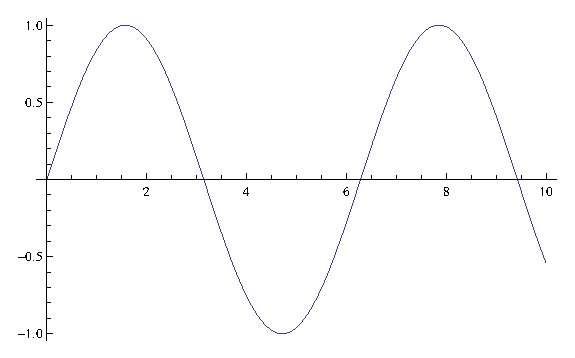
\includegraphics[scale=1]{figures/sin}
  \caption{Plot of $y=sin(x)$}
  \label{fig:sin}
\end{figure}

\begin{figure}[H]
  \centering
    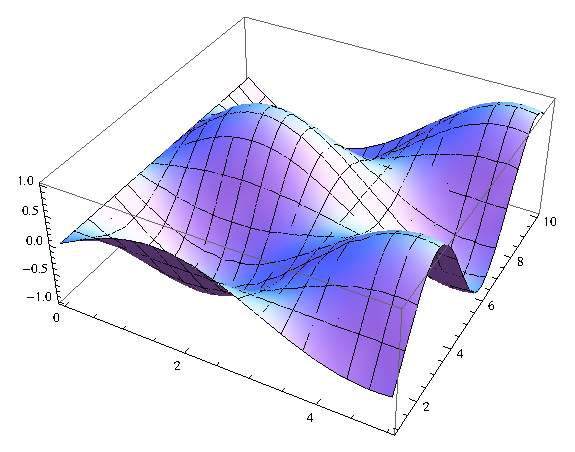
\includegraphics[scale=0.75]{figures/sin3D}
  \caption{Plot of $z=sin(x)cos(y)$}
  \label{fig:sin3D}
\end{figure}

\begin{figure}[H]
  \centering
    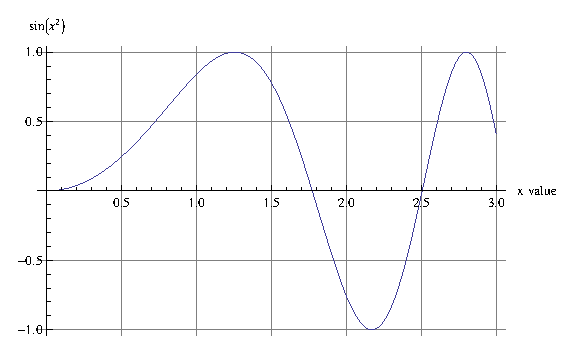
\includegraphics[scale=1]{figures/sinLabel}
  \caption{Plot of $y=sin(x^2)$ with label and axis description}
  \label{fig:sinLabel}
\end{figure}

\subsection{Solving Differential Equation}
Differential equations have three basic types of equations including:
\begin{itemize}
\item \emph{Ordinary Differential Equations} (ODEs), in which there is a single independent variable \textit{t} and one or more dependent variables $x_i(t)$.
\item \emph{Partial Differential Equations} (PDEs), in which there are two or more independent variables and one dependent variable.
\item \emph{Differential-Algebraic Equations} {DAEs}, in which some members of the system are differential equations and the others are purely algebraic, having no derivatives in them.
\end{itemize}

The function \emph{DSolve} gives symbolic solutions to the differential equations while function \emph{NDSolve} generates a general numerical differential equation solver. \emph{DSolve} is powerful in solving ODEs and most first-order PDEs as well as a limited number of the second-order PDEs. For DAEs, it is difficult to find the exact solutions, but \emph{DSolve} can solve many examples of such systems that occur in application.

\subsubsection{Example of solving ODE:}

\begin{figure}[hb]
  \centering
    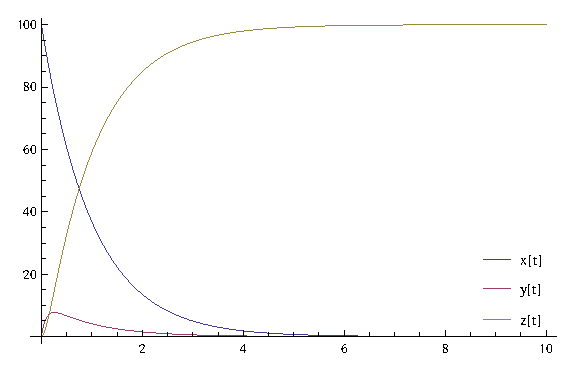
\includegraphics[scale=1]{figures/ODE}
  \caption{Plot of ODE solution}
  \label{fig:ODE}
\end{figure}

\definecolor{light-gray}{gray}{0.95}

%setting
\lstset{
language=Mathematica,
basicstyle=\small\sffamily,
%numbers=left,
%numberstyle=\tiny,
frame=tb,
columns=fullflexible,
showstringspaces=false,
mathescape=true,
escapechar=\@
%backgroundcolor=\color{light-gray}
}

%insert mathematica code
\begin{lstlisting}[caption=ODE solution,
  label=code:ode]
eqns = Join[
{x'[t]== -x[t], y'[t]== x[t] - 10y[t], 
z'[t]== 10y[t],
x[0]==100,y[0]==0, z[0]==0},
{x,y,z}, {t,100}];
sol = NDSolve[eqns];
Plot[
Evaluate[{x[t],y[t],z[t]} /. sol], 
{t,0,10}, 
PlotLegends->Placed[{"x[t]", "y[t]", "z[t]"} , {Right, Bottom}]]
\end{lstlisting}

In this example, we will solve the following ODEs.\\
\begin{equation*}
\left\{
\begin{aligned}
x'[t]&= -x[t],\\
y'[t]&= x[t] - 10y[t],\\
z'[t]&= y[t]
\end{aligned}
\right.
\end{equation*}
where initial conditions are x[0]=100, y[0]=0, z[0]=0 and $t\in[0,100]$.
First, we would use function Join[$list_1, list_2$, ...] to concatenates lists of equations and 
initial conditions into a new list. Then, we use function NDSolve[\textit{eqns}, $u$, {x, $x_{min}$, $x_{max}$}] to compute the numerical solution from the list gotten from Join. Finally, we use function Plot[{$f_1$, $f_2$, ...}, {$x$, $x_{min}$, $x_{max}$}] to draw all the curves of x[t], y[t] and z[t]. The code is as shown in Listing \ref{code:ode} and the curves are shown as Figure \ref{fig:ODE}. For detailed usages of function Join, NDSolve and Plot, please refer to the on-line \emph{Mathematica reference}.




\newtheorem{problem}{Problem}[section]
%\newcommand{\inch}{\ensuremath{\,\textrm{in.}}}

\chapter{One-dimensional Steady State Problems}

\section{Overview}
This Chapter mainly discuss different kind of one-dimensional steady state problems.

\section{Fourier's law}

\begin{example}
\textbf{Fourier’s law, plane wall, constant internal heat
generation.} \textcolor{blue} {\emph{Refer to tutorial Fourier’s
law.nb, and Ch. 2, P. 69.}}

Consider a one-dimensional plane wall in steady state and without heat generation.
Temperature on one side is $T_0=50~K$, other side is $T_1=30~K$, wall width is $L=0.01~m$,
area is $A=1~m^2$, thermal conductivity $k=0.5~W/m.k$. Sketch the heat distribution on T-x coordinate,
what is the heat flux  through the wall?
\end{example}

\begin{solution}
For the plan wall, the heat resistance is
$$R=\frac{L}{kA}$$
So the heat rate 
$$
Q=\frac{\delta T}{R}=kA\frac{T_0-T_1}{L}=1000~W
$$

\begin{lstlisting}
Plot1=Plot[$T_0$ + x/L*($T_1-T_0$),{x, 0, L}]
\end{lstlisting}
The heat flux$$q=\frac{Q}{A}==1000~W/m^2$$
\begin{lstlisting}
R=L/(k*A); (*Resistance*)
$T_0$=50; (*Temperature on the other side of the wall)
$T_1$=30;
Q=($T_0$-$T_1$)/R; (*Watt5s*)
FLUX=Q/A;
\end{lstlisting}
Based on Fourier’s Law, the heat rate
\begin{eqnarray*}
Q=-kA\frac{dT}{dx}\\
dT=-\frac{Q}{ka}dx
\end{eqnarray*}
~\\
Integral
$$\int dT=-\int \frac{Q}{ka} dx$$
In steady state,  is constant, so the heat distribution along the x direction is
$$T(x)=C_1x+C_2$$
As given, $T(0)=T_0=50~K, T(0.01)=T_1=30~K$, we can get
$$T(x)=\frac{T_1-T_0}{L}x+T_0=-2000x+50$$
And the sketch of  is shown below:
\begin{lstlisting}
Plot2=ListPlot[{{0,50},{0.01,30}},
      PlotStyle->{AbsolutePointSize[8]},
      AxesLabel->{Distance (m),Temperature}]
\end{lstlisting}
\end{solution}

\begin{example}
\textbf{Conical section} \textcolor{blue} {\emph{Refer to tutorial 
Prob\_ 7 copy.nb, and Ch. 3, P. 134.}}

A diagram shows a conical section fabricated from pyroceram, $k=3.46W/m.K$.
It is of circular cross section with the diameter $D=ax$, where $a=0.25$.
The small end is at $x_1=50~mm$ and the large end at $x_2=250~mm$.
The end temperature are $T_1=400~K$ and $T_2=600~K$, while the lateral 
surface is well insulated.
\begin{enumerate}
\item Derive and expression for the temperature distribution $T(x)$,
assuming one-dimensional conditions. Sketch the temperature distribution.
\item Calculate the heat rate $Q$ through the cone.
\item If $a$ changes from 0.001 to 1, sketch change of $Q$.
\end{enumerate}
\end{example}

\begin{solution}
\begin{enumerate}
\item
Consider the heat conduction is under steady state, one-dimensional coordinate,
without internal heat generation, the heat transfer rate is a constant independent
of $x$. Use Fourier’s Law to determine the temperature distribution.
$$Q=-kA\frac{dT}{dx}$$
Where $A=\frac{\pi D^2}{4}=\frac{\pi a^2x^2}{4}$. Separating variables,
$$\frac{4Qdx}{\pi a^2x^2}=-kdT$$
Integrating from $x_1$ to any $x$ within the cone, and recalling that $Q$ and $k$
are constant, it follows that
$$\frac{4Q}{\pi a^2}\int_x^{x_1} dx/x^2=-k\int dT$$
Hence
$$\frac{4Q}{\pi a^2}\left(-\frac{1}{x}+\frac{1}{x_1}\right)=-k\left(T-T_1\right)$$
and
$$T(x)=T_1-\frac{4Q}{\pi a^2}\left(\frac{1}{x_1}-\frac{1}{x}\right)$$
Although $Q$ is a constant, it is as yet an unknown.
However, it may be determined by evaluating the above expression at
$x=x_2$, where $T(x_2)=T_2$. Hence
$$Q=\frac{\pi a^2k(T_1-T_2)}{4[(1/x_1)-(1/x_2)]}$$
and solving for Q
\begin{lstlisting}
Q =*a^2*k*(- )/(4((1/x1)-(1/x2))) (*  Watts  *)
\end{lstlisting}
Substituting for $Q$ into the expression for $T(x)$,
the temperature distribution becomes
$$T_2=T_1+(T_1-T_2)\left[\frac{(1/x)-(1/x_2)}{(1/x_1)-(1/x_2)}\right]$$
\begin{lstlisting}
Q =*a^2*k*(- )/(4((1/x1)-(1/x2))) (*  Watts  *)
\end{lstlisting}
From the result, temperature may be calculated as a function of $x$
and the distribution is as shown.
\begin{lstlisting}
Plot2 = Plot[T, {x, .05, .25}, PlotRange -> All, 
AxesLabel -> {Distance (m), Temperature }]
\end{lstlisting}
\item
Substituting numerical values into the foregoing result for the heat 
transfer rate, it follows that
$$Q=\frac{\pi 0.25^2\times3.46~\text{W/m.K}\times(400-600)~K}{4(1/0.05~m - 1/0.25~m)}=-2.12W$$
\item
If changes from $0.001$ to $1$, as $Q$ has expression changes with $a$,
we can sketch $Q$’s changes with $a$.
\begin{lstlisting}
Qax =  *x^2*   k*(- )/(4 ((1/x1) - (1/x2)))
PlotQ = Plot[Qax, {x, .001, 1}, PlotRange -> All,    AxesLabel -> {"a", "Q" }]
\end{lstlisting}
\end{enumerate}
\end{solution}

\section{1-D steady state, constant	internal heat generation problems}
\begin{example}
\textcolor{blue} {\emph{Refer to tutorial HW\_1\_MMATICA.nb}}
A large thin slab of thickness $L=0.1~m$ is “setting.” Setting is an exothermic process 
that releases $\dot{q}=100W/m^3$. Here the slab heat conductivity is in steady state. 
Set the x-axis along with the wall thickness. At position $x=0m$, temperature is $T_0=37~K$,
at position $x=L$,$T_1=33~K$, thermal conductivity $k=0.4W/m.K$. What’s the
temperature distribution in along the length of the slab? 
\end{example}

\begin{solution}
Based on the heat diffusion equation 
$$\nabla^2 T+\frac{\dot{q}}{k}=\frac{1}{\propto}\frac{\partial T}{\partial t}$$
where
$$\nabla^2 T \equiv \frac{\partial^2 T}{\partial x^2}+
\frac{\partial^2 T}{\partial y^2}+
\frac{\partial^2 T}{\partial z^2}$$
In this problem, the large thin slab could be considered as a one-dimensional problem 
with only $x$ dimension, and consider the slab is in steady state with no change with $t$,
so the one-dimensional heat diffusion equation for the slab could be write as
$$\frac{d^2 T}{d x^2}=-\frac{\dot{q}}{k}$$
\begin{lstlisting}
solution1 = NDSolve[{T''[x] + /k == 0, T[0] == ,  T[0.1] == }, T, {x, 0, 0.1}];
\end{lstlisting}
Integration twice
$$T(x)=-\frac{\dot{q}}{2k}x^2+C_1x+C_2$$
By evaluating $T(0)=T_0$, and $T(L)=T_1$, hence
$$T(x)=-\frac{\dot{q}}{2k}x^2+ \left(\frac{T_1-T_0}{L}+\frac{\dot{q}L}{2k}\right)x+T_0$$
From the result, temperature distribution could be expressed as a quadratic curve as below
\begin{lstlisting}
PS1 = Plot[Evaluate[T[x] /. First[solution1]], {x, 0, 0.1},    PlotRange -> All]
\end{lstlisting}
\end{solution}

\begin{example}
\textcolor{blue} {\emph{Refer to tutorial HW\_1\_MMATICA.nb, and Ch. 3, P. 134.}}
~\\
A steady state long tube generating thermal energy at a uniform volumetric rate
$\dot{q}=1000W/m^3$, the thermal conductivity $k=0.4$W/m.K.
At radius $r_1=0.1368m$, temperature $T_0=37~K$, at position $r_2=0.1768m$
, temperature $T_1=33~K$, the two end of the rod are well insulated.
What is the temperature distribution along the radius of the tube?
\end{example}

\begin{solution}
The heat diffusion equation for cylindrical system is 
$$ 
\frac{1}{r}\frac{\partial}{r}(kr\frac{\partial T}{\partial r})+
\frac{1}{r^2}\frac{\partial}{\phi}(k\frac{\partial T}{\partial \phi})+
\frac{\partial}{z}(k\frac{\partial T}{\partial z})+
\dot{q} =
\rho c_p\frac{\partial T}{\partial t}
$$
In this problem, consider the heat distribution change only on $r$ direction,
and since the tube is in steady state, the temperature distribution would not
change with time $t$. The heat distribution equation could be written as
$$\frac{1}{r}\frac{\partial}{r}(kr\frac{\partial T}{\partial r})+\dot{q}=0$$
Integration twice
$$T(r)=-\frac{\dot{q}}{4k}r^2+C_1Inr+C_2$$
Substituting $T(r_1)=T_0$, $T(r_2)=T_1$, hence
$$
T(r)=-\frac{\dot{q}}{4k}r^2 +\left[\frac{T_1-T_0+(\dot{q}/4k)\cdot r_2^2}{In(r_2/r_1)} \right]\cdot Inr +
\frac{T_0Inr_2-T_1Inr_1-(\dot{q}/4k)\cdot r_2^2}{In(r_2/r_1)}
$$
~\\
By evaluating $r_1=0.1368~m, T_0=37~K, r_2=0.1768~m \text{and} T_1=33~K$,
sketch the $T(r)$
\end{solution}

\section{1-D steady state, variate internal	heat generation	problems}

\section{Fin problems}
\begin{example}
A rectangular fin with uniform cross-sectional area has constant heat conductivity 
$k=3~W/m.K$ heat conduction coefficient $h=10~W/mc$, width is $W=0.01~m$, 
Thickness is $L=1~m$. At start position $x_1=0~m$, temperature is $T_1=30^\circ C$.
The surface of the fin is exposed to ambient air at $10~K$ with a convection heat transfer
coefficient $h=10~W/m^2K$. Plot the temperature distribution in the fin under below conditions.
\begin{enumerate}
\item Prescribed tip temperature: at the end position $x_2=0.04m, T_2=40^\circ C$
\item Adiabatic tip condition.
\item Infinite tip condition.
\end{enumerate}

\end{example}

\begin{solution}
~\\
\begin{enumerate}
\item
The fin energy balance equation
$$$$
For the proscribed fin problem with constant cross section area , and surface area, we have  ,  . Hence 

To simplify the form of this eqauation, we transform the dependent variable by defining an excess temperature  as 

Where since  is constant, . Then we obtain

Where 

With prescribed boundrary condition

Then for prescribed condition the fin temperature distribution is
\item

For adiabatic tip condition, the heat convection rate at the tip is considered negligible,

And 

Then the heat distribution equation of adiabatic tip condition could be written as

The temperature distribution along x direction is shown below
\item
For an infinite fin the tip is , and the boundary condition at the tip is 

And the temperature distribution is 

Sketch the temperature distribution 
\end{enumerate}

\end{solution}

\begin{example}
\textbf{Constant k and A}
A rectangular fin with uniform cross-sectional area has constant heat conductivity heat conduction coefficient , width is , Thickness is . At start position , temperature is . The surface of the fin is exposed to ambient air at  with a convection heat transfer coefficient . Plot the temperature distribution in the fin under below conditions.
\end{example}

\begin{solution}
TODO
\end{solution}



\chapter{Two-dimensional Steady State problems}
\section{Overview}
This section we mainly introduce the method to solve two dimensional steady state problems, the example given introduces how to calculate the temperature distribution in square steady heat conduction problem without internal heat generation, and how to calculate the heat flux in the square.
\section{Exact Solution}
\begin{example}
\textcolor{blue} {\emph{Refer to 3-2-1Two dimenstional steady state not heat generation.nb.}}
A two-dimensional rectangular plate length and width is $L=2$,$W=1$, and on one 
boundary temperature $T_2=150~K$, other three boundaries $T_2=50~K$. The square 
is in steady state, sketch the temperature distribution and temperature at position $x=1$ and $y=0.5$,
Calculate the heat flux when $y=0$. (As shown in figure \ref{fig:3:1})
\begin{figure}[h!]
  \centering
    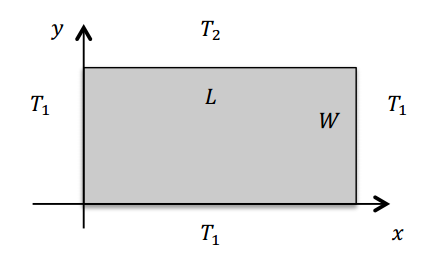
\includegraphics[scale=0.8]{figures/ch3/1}
    \caption{Model of Example3.2.1}
    \label{fig:3:1}
\end{figure}
\end{example}

\begin{solution}
To simplify the solution, use below transformation
$$\theta=\frac{T-T_1}{T_2-T_1}$$
According to heat diffusion equation, the two-dimensional, steady state with no internal heat generation equation is 
$$\frac{\partial^2 T}{\partial x^2}+\frac{\partial^2 T}{\partial y^2}=0$$
the transformed differential equation is then
$$\frac{\partial^2 \theta}{\partial x^2}+\frac{\partial^2 \theta}{\partial y^2}=0$$
Since the equation is second order in both x and y, two boundary conditions are needed for each of the coordinates, they are
$$\theta(0,y)=0,\text{and}  \theta(x,0)=0$$
$$\theta(L,y)=0,\text{and}  \theta(x,W)=1$$
The $\theta(x,y)$ is
$$\theta(x,y)=\frac{2}{\pi}\sum\limits_{i=1}^\infty 
\frac{(-1)^{n+1}+1}{n}\sin{\frac{n\pi x}{L}}
\frac{\sinh{n\pi y/L}}{\sinh{n\pi W/L}}
$$
So that 
$$T(x,y)=(T_2-T_1)\frac{2}{\pi}\sum\limits_{i=1}^\infty 
\frac{(-1)^{n+1}+1}{n}\sin{\frac{n\pi x}{L}}
\frac{\sinh{n\pi y/L}}{\sinh{n\pi W/L}}+T_1
$$
Plot 3D sketch of the temperature distribution in the rectangular is shown as Figure\ref{fig:3:2}
\begin{figure}[h!]
  \centering
    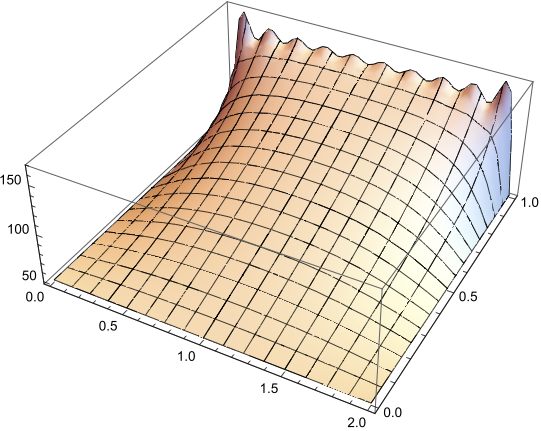
\includegraphics[scale=0.8]{figures/ch3/2}
    \caption{Temperature distribution in square with series method}
    \label{fig:3:2}
\end{figure}

And by fixing $x$ and $y$ separately we can get the temperature distribution $T(1,y)$ as Figure \ref{fig:3:3} and $T(x,0.5)$ as Figure \ref{fig:3:4}
\begin{figure}[h!]
  \begin{minipage}[b]{0.45\linewidth}
  \centering
    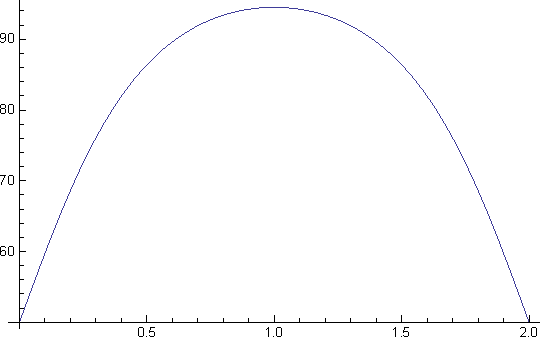
\includegraphics[scale=0.7]{figures/ch3/3}
    \caption{Temperature distribution in square at $x=1$}
    \label{fig:3:3}
\end{minipage}
\hspace{0.5cm}
\begin{minipage}[b]{0.45\linewidth}
  \centering
    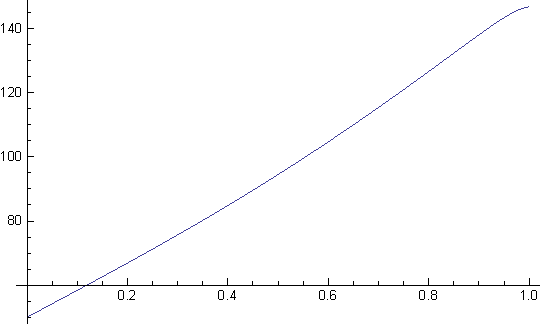
\includegraphics[scale=0.7]{figures/ch3/4}
    \caption{Temperature distribution in square at $y=0.5$}
    \label{fig:3:4}
\end{minipage}
\end{figure}
To calculate the heat flux passing through a unique section line, we use Fourier's equation $q=-kA(\partial T/\partial x\partial y)$ for heat rate at point $(x, y)$. When $y=0$, the heat flux passing through $x$ direction in the square could be represented as

\begin{equation*}
\begin{aligned}
Q&=\int_0^L \! Aq \, \mathrm{d} x|_{y=0} \\
&=2kA(T_2+T_1)\sum\limits_{i=1}^\infty 
\cosh{\frac{(2n-1)\pi y}{2}}\csc{\frac{(2n-1)\pi}{2}}\sin{\frac{(2n-1)\pi x}{2}}|_{y=0}
\\&=8346.27
\end{aligned}
\end{equation*}


\end{solution}





\chapter{Transient conduction problems}
\section{Overview}
\section{The lumped capacitance method}


\begin{appendices}
%\addcontentsline{toc}{\chapter}{Appendices}
\appendixpage
\noappendicestocpagenum
\addappheadtotoc

\newcommand{\myWSEgPath}[1] {
\label{example:#1}
  \textcolor{blue} {(Please refer to .../workshopNB/#1.nb)}}

\renewcommand{\thesection}{\arabic{section}}

\chapter*{Mathematica Workbook Listing*}
~\\Here is a listing of most common seen heat transfer condition and regularly used methods for solving the problems. As listed, the problem marked with \textbf{*} were already mentioned in the tutorial examples. Others will be further discussed in the mathematica workbooks.

\section*{General topics*}

\begin{itemize}
\item Steady State: $\nabla^2T+\frac{q'''}{k}=0$
\begin{itemize}
\item 1-D: Fourier's Law*
\item 1-D: Geometry: Cartesian*, Cylindrical, Spherical
\item 1-D: with heat generation
\item Special 1-D and Fin Solutions:
\begin{itemize}
\item Variable X-S area*
\item Fin: Cartesian*
\item Fin: Radial
\item Bioheat Equation (Fin analog)*
\end{itemize}
\end{itemize}

\item Multi-dimensional: $\nabla^2T+\frac{q'''}{k}=0$
\begin{itemize}
\item 2-D: Exact solution rectangle*
\begin{itemize}
\item Derivative on a boundary (heat flux)*
\end{itemize}
\item NDSolve with heat generation?
\end{itemize}

\item Transient: $\frac{1}{\alpha}\frac{\partial T}{\partial t}
=\nabla^2T+\frac{q'''}{k}$
\begin{itemize}
\item Lumped form*
\begin{itemize}
\item Special case –radiative condition (lumped system HMWK4P7)
\end{itemize}
\item (Lumped vs. Transient 1 term – HMWK4P4 or other)*
\item SOV*–  Case 9 – analytical solution (Ozisik Table 2.1)
\item NDSolve\^: 1 Dheat(WORKS) (w/ and w/o g) can compare to SOV
\item Semi-infinite solutions
\end{itemize}


\item Numerical (Programming in Mathematica)
\begin{itemize}
\item Finite difference Fin*
\item Finite Difference Cartesian, Cylindrical and Spherical (Fin Diff 3 geometries)
\end{itemize}

\end{itemize}

\section*{Specific topics \uppercase\expandafter{\romannumeral1}}
See Mathematica 1999 Tutorial (See Conduction Problems Folder).
\begin{itemize}
\item Multi-dimensional SOV solutions \\
(See:  Tutorial: Mathematica for Advanced Heat Transfer)
\begin{itemize}
\item Cartesian
\item Cylindrical
\item Spherical
\end{itemize}

\item Laplace Solution

\end{itemize}

\section*{Specific topics \uppercase\expandafter{\romannumeral2}}
\begin{itemize}
\item Drug Delivery
\begin{itemize}
\item One compartment drug delivery
\item Two compartment drug delivery
\end{itemize}
\item Phase Change (Xiaoqing)
	\begin{itemize}
	\item Part \uppercase\expandafter{\romannumeral1}: Steady State
	\item Part \uppercase\expandafter{\romannumeral2}: Quasi – Steady Solutions (Cooper and Trezek)
	\item Part \uppercase\expandafter{\romannumeral3}: Neumann + Stefan
	\end{itemize}
\item Biophysics
	\begin{itemize}
	\item Arrhenius Modeling vs. Clinical Equivalent Minutes (CEM)
		\begin{itemize}
		\item Protein denaturation \& Fractional denaturation
		\item Thermal Dose
		\end{itemize}
	\item Water Transport
	\item Cryoprotective Loading
	\end{itemize}
\item Iron Oxide Nanoparticle Heating
	\begin{itemize}
	\item Cancer
	\item Regenerative Medicine (See Navid)
	\end{itemize}

\end{itemize}





\chapter{General Topics}
%\renewcommand{\thechapter}{\arabic{chapter}}

%\addcontentsline{titletoc}{part}{\appendixname}
\numberwithin{example}{section}
%\chapter{Workshops examples*}



\section{1-dimensional steady state}
\subsection{Variable heat generation}
\begin{example}
\textbf{1-D steady state solution in Cartisian coordinate}\\
BCs: at $x=0$, $T=10$; 
$x=1$, $T=100$ Heat Generation: g variable Given: $k=1$
\myWSEgPath{1-1}
\begin{figure}[H]
  \centering
    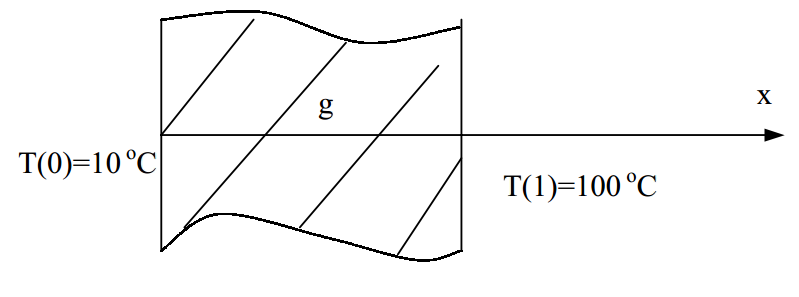
\includegraphics[scale=0.5]{figures/appendixA/1}
\end{figure}
$$T''+g=0$$
$$T=0.5gx^2+C_1x+C_2$$
\end{example}

\subsection{Spehrical coordinate}
\begin{example}
\textbf{1 - D steady state solution in spherical coordinate}\\
BCs: at $r = 0.1$, $T = 10$; $r = 1$, $T = 100$.
Heat Generation: g variable
\myWSEgPath{1-2}
Given: $k=1$
\begin{figure}[H]
  \centering
    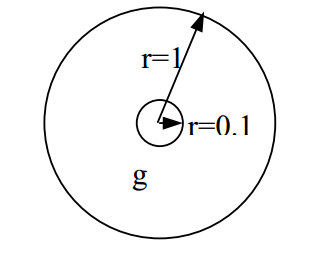
\includegraphics[scale=0.5]{figures/appendixA/2}
\end{figure}
$$\frac{1}{r}\frac{d^2}{dr^2}(rT)+g=0$$
$$T=\frac{1}{6}gr^2+\frac{C_1}{r}+C_2$$
\end{example}

\subsection{round fin}
\begin{example}
\textbf{fin problem: round rod}\\
Given: $k=206W/m/K$
\myWSEgPath{1-3}
\begin{figure}[H]
  \centering
    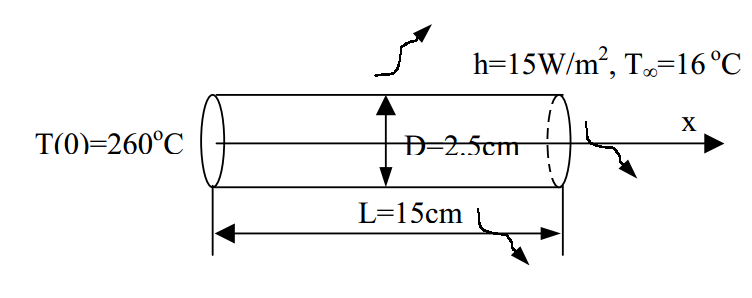
\includegraphics[scale=0.5]{figures/appendixA/3}
\end{figure}
$$\theta=T-T_\infty$$
$$\theta''-m^2\theta=0,~m=\sqrt{\frac{hp}{kA}}$$
$$\theta=\frac{\cosh{m(l-x)}+n\sinh{(m(l-x))}}{\cosh{(ml)}+n\sinh{(ml)}}\theta_0,~n=h/(km)$$
\end{example}

\section{Multi-dimensional steady state}
\subsection{2D square with heat generation, NDSolve method}

\section{Transient}
\subsection{Lumped form cylindrical}
\begin{example}
\textbf{lumped problem:long thin rod at $T(0)=20^oC$}\\
Given: $k = 0.5$; $\rho= 900$; $C_p = 3800$.
\myWSEgPath{2-1}
\begin{figure}[H]
  \centering
    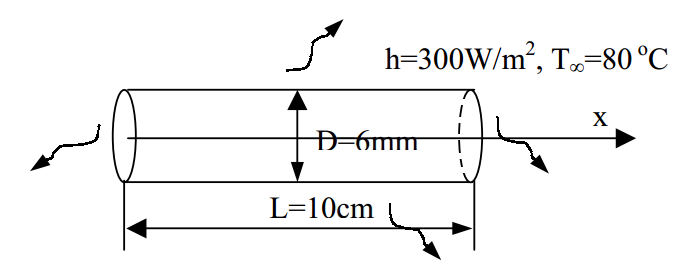
\includegraphics[scale=0.5]{figures/appendixA/4}
\end{figure}
$$\theta=T-T_\infty$$
$$\theta'-m^2\theta=0,~m=\sqrt{\frac{hA}{\rho C_pV}}$$
$$\theta=\theta_0e^{-mt}$$
\end{example}
\subsection{Lumped form radiative condition}

\subsection{SOV method: Catesian, Cylindrical, Spherical}
\begin{example}
\textbf{ SOV (separation of variable) in 1D Cartisian space and time
No heat Generation}\\
$k = 0.5$; $\rho=1000$; $C_p = 4200$.
\myWSEgPath{2-2}
\begin{figure}[H]
  \centering
    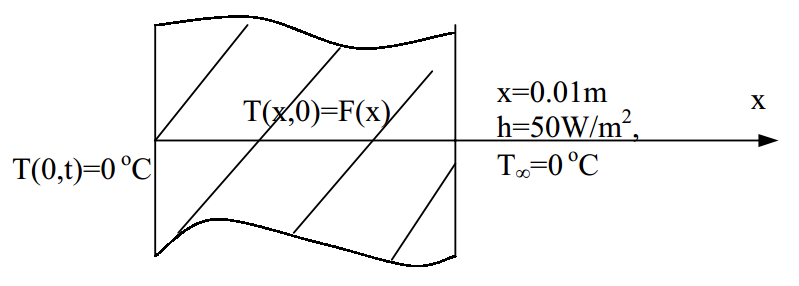
\includegraphics[scale=0.5]{figures/appendixA/5}
\end{figure}

$$\frac{\partial T}{\partial t}=
\alpha\left(\frac{\partial^2 T}{\partial x^2}+
\frac{\partial^2 T}{\partial y^2}+
\frac{\partial^2 T}{\partial z^2}\right)$$
$$T(x,t)=X(x)Y(y)Z(z)\Gamma(t)$$
$$X(x),~Y(y),~\text{and} ~Z(z)\text{: trigonometric function}$$
$$\Gamma(t)\text{: exponential decay function}$$
$$\text{Trigonometric differential equation: }X''+\beta^2X=0$$
$$T=\sum_{i=1}^{\infty} \frac{1}{N_i}e^{-\alpha{\beta_i}^2t}\sin{(\beta_i x)}\int_0^{l}\sin{(\beta_i x')}F(x')dx'$$
$$\beta\cot{(\beta l)}=-h/k$$
$$\frac{1}{N_i}=2\frac{{\beta_i}^2+{H_2}^2}{l({\beta_i}^2+{H_2}^2)+H_2},
~H_2=h/k$$
\end{example}
\begin{example}
\textbf{SOV (separation of variable) in 1D Cylindrical space and time
No heat Generation}
$k = 0.5$; $\rho= 1000$; $C_p = 4200$.
\myWSEgPath{2-3}
\begin{figure}[H]
  \centering
    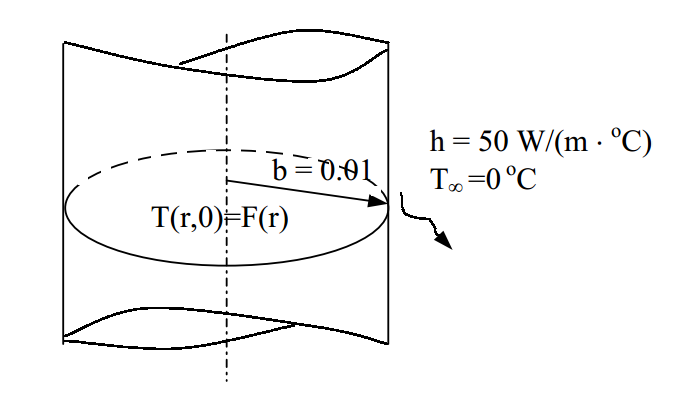
\includegraphics[scale=0.5]{figures/appendixA/6}
\end{figure}
$$\frac{1}{\alpha}\frac{\partial T}{\partial t}=
\frac{\partial^2 T}{\partial z^2}+
\frac{1}{r^2}\frac{\partial^2 T}{\partial \phi^2}+
\frac{1}{r}\frac{\partial T}{\partial r}+
\frac{\partial^2 T}{\partial r^2}$$
$$T(z,r,\phi,t)=Z(z)R(r)\Phi(\phi)\Gamma(t)$$
$$Z(z)~\text{and} ~\Phi(\phi)\text{: trigonometric}$$
$$R(r)\text{: Bessel function}$$
$$\Gamma(t)\text{: exponential decay function}$$
$$\text{Bessel differential equation (order } \upsilon\text{):}
\frac{\partial^2 R}{\partial r^2}+
\frac{1}{r}\frac{\partial R}{\partial r}+
\left(\beta^2-\frac{\upsilon^2}{r^2}\right) R=0
$$

$$\upsilon \text{ is eigenvalue of trigonometric differential equation of } \Phi(\phi)$$
$$T(r,t)=\sum_{i=1}^{\infty} \frac{1}{N_i}e^{-\alpha{\beta_i}^2t}J_\upsilon(\beta r)\int_0^{b}r'J_\upsilon(\beta r')F(r')dr'$$
$$0.5\beta(J_{\upsilon-1}(\beta b)-
J_{\upsilon+1}(\beta b))+
HJ_{\upsilon+1}(\beta b)=0,
~H=h/k
$$
$$\frac{1}{N_i}=\frac{2}{J_\upsilon(\beta b)}
\frac{\beta^2}{b^2(\beta^2+H^2)-\upsilon^2}
$$
\end{example}

\begin{example}
\textbf{SOV (separation of variable) in 1D spherical space and time: full sphere No heat Generation}\\
$k = 0.5$, $\rho= 1000$, $C_p = 4200$, $b=0.01$, $T(x,0)=60$, $T(b,t)=0$.
\myWSEgPath{2-4}
\begin{figure}[H]
  \centering
    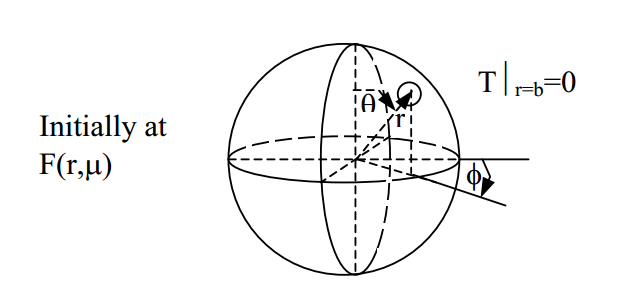
\includegraphics[scale=0.5]{figures/appendixA/7}
\end{figure}
$$ 
\frac{1}{\alpha}\frac{\partial T}{\partial t}=
\frac{\partial^2 T}{\partial r^2}+
\frac{2}{r}\frac{\partial T}{\partial r}+
\frac{1}{r^2\sin \theta} \frac{\partial}{\partial \theta}
\left( \sin\theta\frac{\partial T}{\partial \theta} \right)
+\frac{1}{r^2{\sin{\theta}}^2}\frac{\partial^2 T}{\partial \phi^2}
$$
$$\mu=\cos \theta,~V=r^{0.5}T$$
$$
\frac{1}{\alpha}\frac{\partial V}{\partial t}=
\frac{\partial^2 V}{\partial r^2}+
\frac{1}{r}\frac{\partial V}{\partial r}-
\frac{V}{4r^2}+
\frac{1}{r^2}\frac{\partial}{\partial \mu}
\left( (1-\mu^2)\frac{\partial V}{\partial \mu}\right)+
\frac{1}{r^2(1-\mu^2)}\frac{\partial^2 V}{\partial \phi^2}
$$

$$V(r,\mu,\phi,t)=R(r)M(\mu)\Phi(\phi)\Gamma(t)$$
$$R(r)\text{: Bessel function, }\beta$$
$$\Phi(\phi)\text{: trigonometric, m}$$
$$\Gamma(t)\text{: exponential decay function}$$
$$M(\mu)\text{: Legendre polynomial}$$
$$ 
\frac{\partial^2 R}{\partial r^2}+
\frac{1}{r}\frac{\partial R}{\partial r}+
\left(\beta^2-\frac{(n+0.5)^2}{r^2}\right) R 
=0\text{, order n+0.5 Bessel differential equation}
$$
$$
\frac{\partial}{\partial \mu}
\left( (1-\mu^2)\frac{\partial V}{\partial \mu}\right)+
\left[ n(n+1)-\frac{m^2}{1-\mu^2} \right]M=0
$$
$$\text{Legendre’s associated differential equation of degree n and order m}$$
\begin{equation*}
\begin{aligned}
T(r,\mu,t)=&\sum_{n=0}^{\infty}\sum_{p=1}^{\infty} \frac{1}{N(n)N(\beta_{np})}
e^{-\alpha{\beta_{np}}^2t}r^{-0.5}J_{n+0.5}(\beta_{np}r)P_n(\mu)\times\\
&\int_{r'=0}^{b}\int_{\mu'=-1}^{1} {r'}^{1.5}J_{n+0.5}(\beta_{np}r')P_n(\mu')F(\mu',r')d\mu'dr'
\end{aligned}
\end{equation*}
$$J_{n+0.5}(\beta_{np}b)$$
$$N(n)=\frac{1}{2n+1}$$
$$N(\beta_{np})=-\frac{b^2}{2}J_{n-0.5}(\beta_{np}b)J_{n+1.5}(\beta_{np}b)$$
\end{example}

\begin{example}
\textbf{SOV (separation of variable) in 1D spherical space and time: half sphere}. \myWSEgPath{2-5}
\begin{figure}[H]
  \centering
    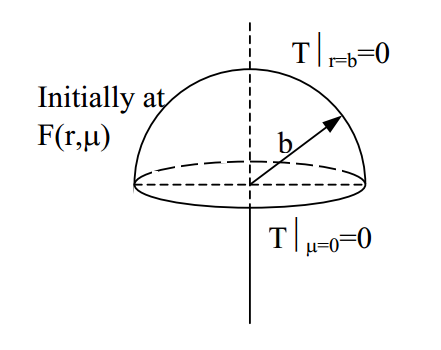
\includegraphics[scale=0.5]{figures/appendixA/8}
\end{figure}
\begin{equation*}
\begin{aligned}
T(r,\mu,t)=&\sum_{n=1,3,5\dots}^{\infty}\sum_{p=1}^{\infty} \frac{1}{N(n)N(\beta_{np})}
e^{-\alpha{\beta_{np}}^2t}r^{-0.5}J_{n+0.5}(\beta_{np}r)P_n(\mu)\times\\
&\int_{r'=0}^{b}\int_{\mu'=-1}^{1} {r'}^{1.5}J_{n+0.5}(\beta_{np}r')P_n(\mu')
F(\mu',r')d\mu'dr'
\end{aligned}
\end{equation*}

$$J_{n+0.5}(\beta_{np}b)$$
$$N(n)=\frac{1}{2n+1}$$
$$N(\beta_{np})=-\frac{b^2}{2}J_{n-0.5}(\beta_{np}b)J_{n+1.5}(\beta_{np}b)$$
\end{example}

\begin{example}
\textbf{Semi-infinite domain solution: error function and complimentary error
function}\\
$k = 0.5$, $\rho= 1000$, $C_p = 4200$.
Initial condition: $T(x,0)=0$
Boundary condition: $T(0,t)=100^oC$ or convective $w/:h=100w/m^2$, $T_f=100^oC$.\myWSEgPath{2-6}
\begin{figure}[H]
  \centering
    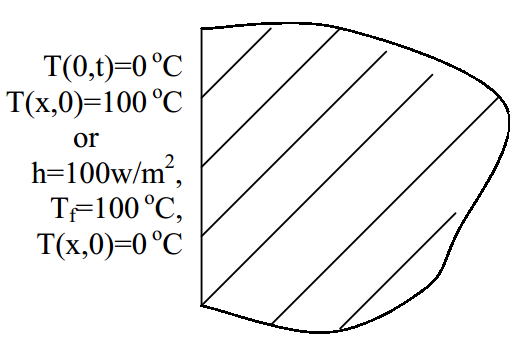
\includegraphics[scale=0.5]{figures/appendixA/9}
\end{figure}
$$T(x,t)=T_0 erf(x/\sqrt{4\alpha t}),~T(0,t)=0^o C\text{ or,}$$
\begin{eqnarray*}
&T(x,t)=T_0 erfc(x/\sqrt{4\alpha t})-e^{Hx+H^2\alpha t}
erfc(H \sqrt{\alpha t}+x\sqrt{4\alpha t})\\
&\text{ for convective conditions}
\end{eqnarray*}
\end{example}

\subsection{NDSolve method}

\subsection{Semi-infinite solutions}
\begin{example}
\textbf{Analytical solution}
\end{example}

\begin{example}
\textbf{Duhamel method}
\end{example}

\begin{example}
\textbf{Laplace method}
\end{example}

\subsection{Numerical method}
\begin{example}
\textbf{Finite Difference method for fin: Cartesian, Cylindrical and Spherical}
\end{example}

\chapter{Special Topics \uppercase\expandafter{\romannumeral1}}
\section{Multi-dimensional SOV solutions}

\begin{example}
\textbf{Finite Difference method for fin: Cartesian, Cylindrical and Spherical}
\end{example}

\section{Laplace Solution}
\begin{example}
\textbf{Laplace Solution}
\end{example}

\section{Duhamel Solution}
\begin{example}
\textbf{DuhamelSolution}
\end{example}

\section{More Error Function Solutions}
\begin{example}
\textbf{Semi Inf. Domain}
\end{example}

\chapter{Special Topics \uppercase\expandafter{\romannumeral2}}

\section{Drug Delivery}
\begin{example}
\textbf{One compartment drug delivery}
\end{example}

\begin{example}
\textbf{Two compartment drug delivery}
\end{example}

\section{Phase Change}
\begin{example}
\textbf{Part I: Steady State}
\end{example}

\begin{example}
\textbf{Part II: Quasi – Steady Solutions (Cooper and Trezek)}
\end{example}

\begin{example}
\textbf{Part III:  Neumann + Stefan}
\end{example}

\section{Biophysics}
\subsubsection{Arrhenius Modeling vs. Clinical Equivalent Minutes (CEM)}
\begin{example}
\textbf{Protein denaturation \& Fractional denaturation}
\end{example}

\begin{example}
\textbf{Thermal Dose}
\end{example}

\subsection{Water Transport}
\subsection{Cryoprotective Loading}

\section{Iron Oxide Nanoparticle Heating}

\begin{example}
\textbf{Cancer}
\end{example}

\begin{example}
\textbf{Regenerative Medicine}
\end{example}

\end{appendices}

\bibliographystyle{plain}
\bibliography{bibliography/MathematicaTutorial}
\end{document}